\appendix

\section{Data Plans around the World}\label{Dataplans}

In most countries, the dominant forms of mobile data pricing are still usage-based or tiered. However, the actual cost of mobile data can vary greatly from country to country, depending on such factors as the country's network infrastructure, market competition, and population density. One common distinction is between pre- and postpaid plans.\footnote{Prepaid plans are those in which a consumer pays for his/her data usage beforehand, while for postpaid plans, a consumer is billed for his/her monthly usage at the end of the billing cycle.} Castells et al. \cite{castells2007mobile} found a strong correlation between the availability of prepaid plans for voice calls and adoption rates of mobile telephone subscribers, which is corroborated by Hauge et al. \cite{hauge2009whose}.  In this Appendix, we provide an overview of prepaid and postpaid plan adoption in different parts of the world and its relationship to consumer market demographics.

\begin{figure}
\centering
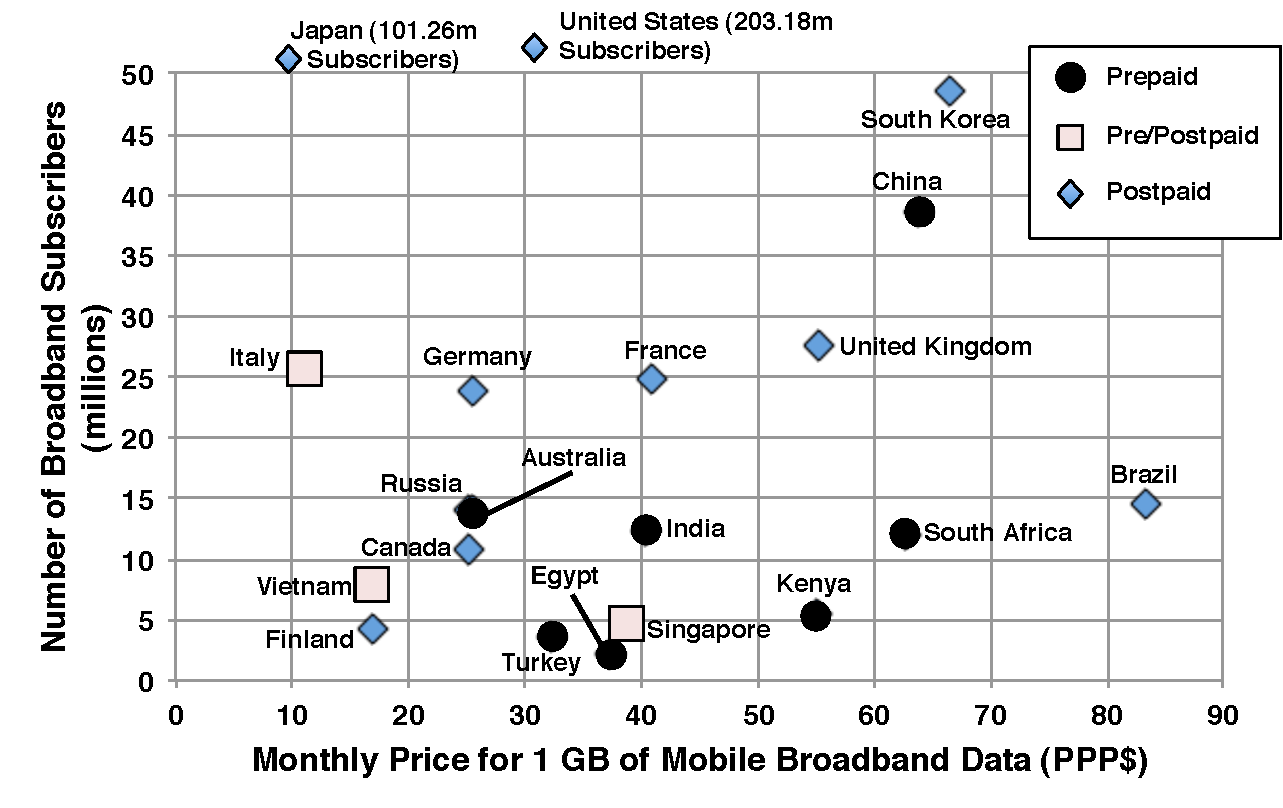
\includegraphics[width=0.75\textwidth]{Figures/World.pdf}
\caption{Prepaid and postpaid mobile broadband data plans around the world (data from 2011).  Data were taken from operator websites as well as \cite{chinamobile,SAfrica,cia,kenyatotal,egypttotal,singapore,itu,italy,india,docomo,oecd,chinatotal,russiatotal,braziltotal,korea,vietnamtotal,worldbank}.}
\label{fig:world}
\end{figure}

\begin{figure}
\centering
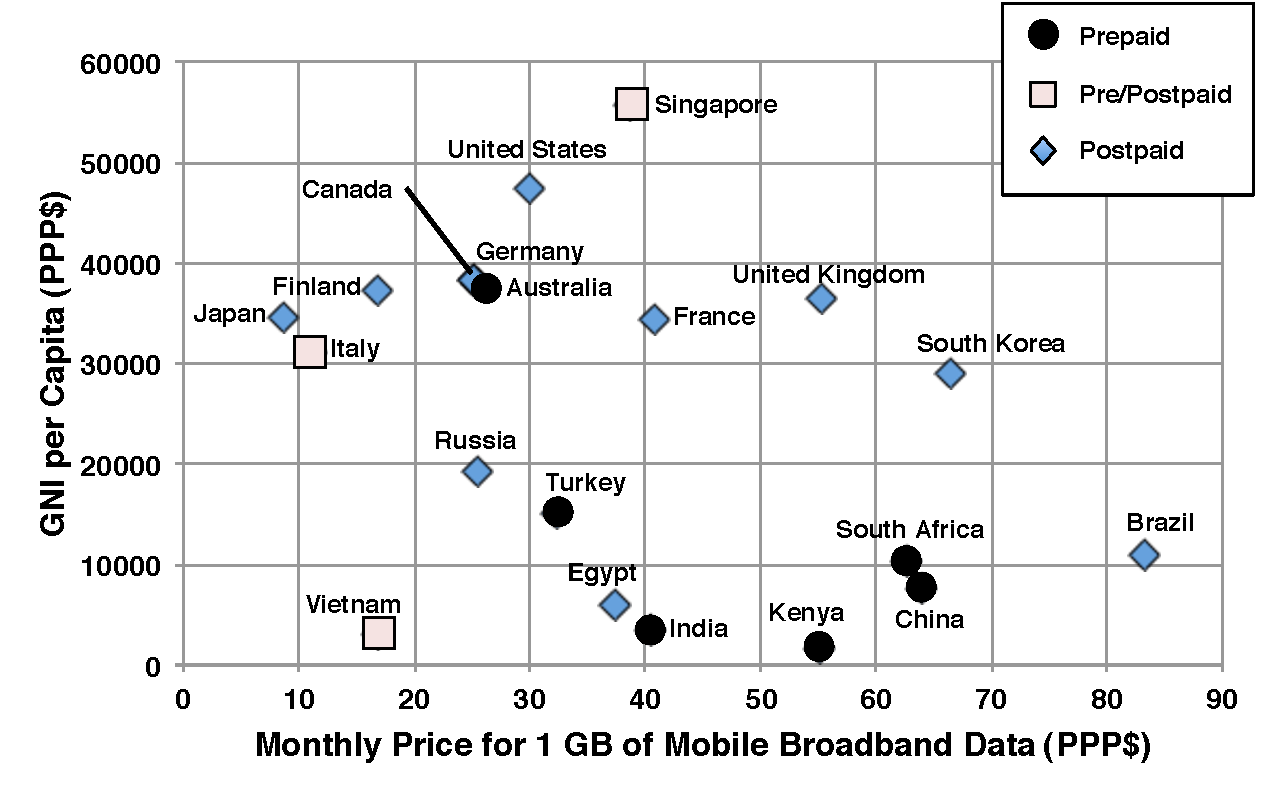
\includegraphics[width=0.75\textwidth]{Figures/GNI.pdf}
\caption{GNI per capita vs. monthly cost of 1GB of mobile data (data sources as in Figure \ref{fig:world}).}
\label{fig:gni}
\end{figure}

\begin{figure}
\centering
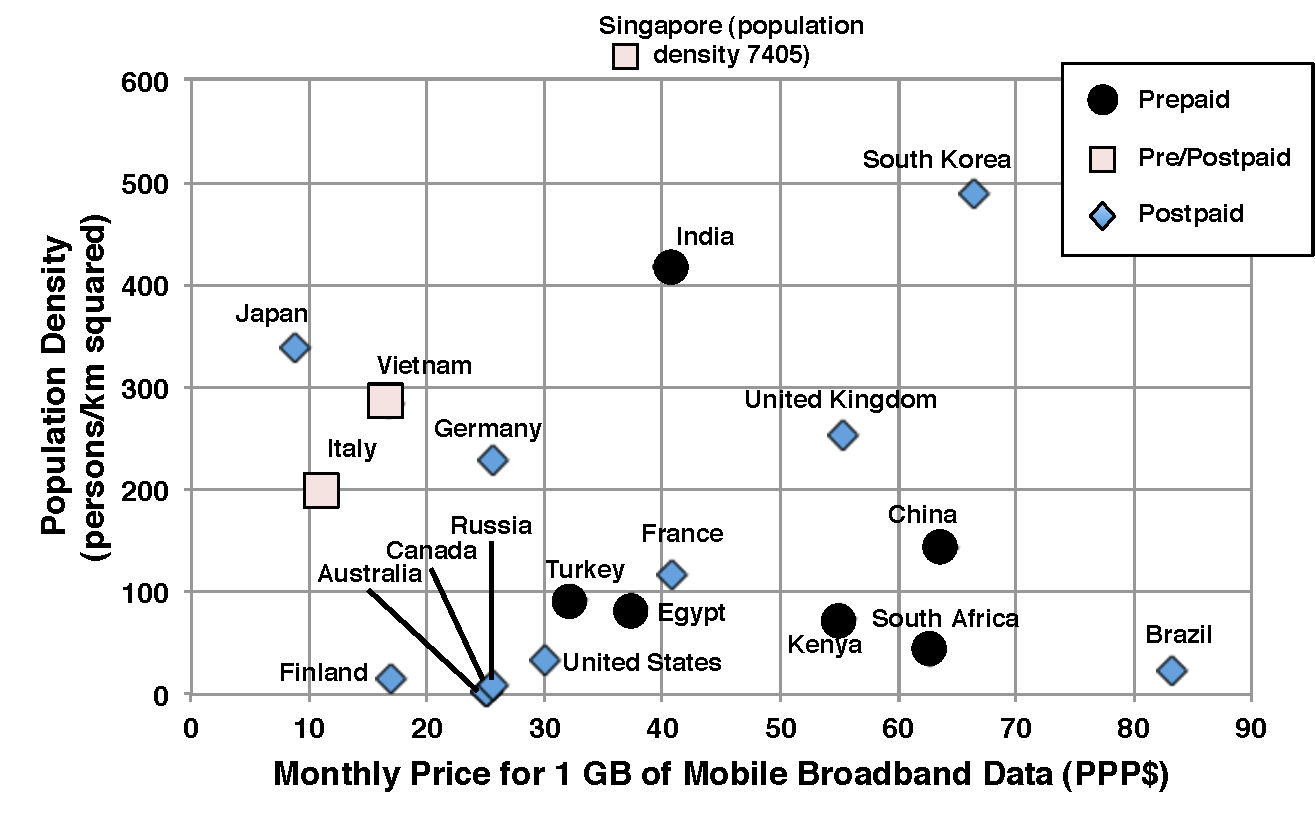
\includegraphics[width=0.75\textwidth]{Figures/Density_PPP.pdf}
\caption{Population density vs. monthly cost of 1GB of mobile data (data sources as in Figure \ref{fig:world}).}
\label{fig:density}
\end{figure}

Figure \ref{fig:world} shows whether prepaid or postpaid plans are the dominant form of data plans in several countries of the world, as of 2011. To determine this data, we examined the standard mobile subscriptions for the largest mobile operator in each country and plotted the monthly cost (in \$ after accounting for purchasing power parity) of 1GB of data usage.  We note that the data plans in different countries have different broadband caps, which are not reflected in the graph, but may be found in \cite{itu}. The cost of 1GB of data/month has been plotted against the number of mobile broadband subscribers in each country; we observe that there is a large variation in cost. Additionally, we see that the countries of Africa (e.g., Kenya, South Africa), the Middle East (e.g., Turkey, Egypt), India and China tend to prefer prepaid plans, while postpaid plans dominate in Europe and the Americas. There is a weakly positive correlation between the price for mobile data and the number of broadband subscribers in the country.

Figure \ref{fig:gni} more explicitly shows the correlation between prepaid mobile broadband data plans and lower per capita gross national incomes (GNI): we see that countries with a lower GNI per capita tend to have prepaid plans as the dominant subscription mode, with the exception of Australia.  Moreover, two of the three countries offering both pre- and postpaid plans (Italy and Vietnam) have GNI per capita below the wealthiest 9 countries. Wealthier countries tend to have lower prices for mobile data, even accounting for purchasing power parity. In lower-GNI countries, it is possible that only a wealthy subset who can afford higher prices generally purchase mobile data plans; another explanation is that these countries have lower investment costs due to their relative wealth.

Infrastructure development is also related to population density: in denser countries, networks need to cover a smaller geographical area to reach the same number of people, resulting in lower investment costs. In the rural United States, small carriers often cite wireline backhaul over long distances as a major source of wireless network costs \cite{neca}. Figure \ref{fig:density} shows a negative correlation between population density and the price for 1GB of mobile data, consistent with our hypothesis that denser countries have lower infrastructure costs. Prepaid data plans are somewhat more popular in less dense countries, with India a notable exception: 83\% of countries with prepaid plans have lower population density than 36\% of countries with high population density and postpaid data plans. These countries also tended to have lower GNIs, which along with their population density suggest that their network infrastructure is less comprehensive than that of denser, wealthier countries.

% Within the U.S., prepaid data plans have gained popularity due to their lower, shorter-term financial commitment and relative simplicity compared to postpaid usage-based pricing plans with data caps.  Moreover, operators are offering more attractive prepaid devices with data-centric plans that appeal to young, price-sensitive users \cite{pcworld}.

%\section{Coping with Usage-based Pricing}
%
%While usage-based pricing is one of the simplest pricing plans, besides charging flat fees for unlimited usage, a major limitation to usage pricing is that many people do not understand how much data their applications use. Thus, even tiered data plans with monthly caps can be hard for them to manage. Several user apps have been developed to 